\documentclass[manuscript,review,anonymous]{acmart}

%% ------------------------------------------------------------------
%% BASiS 日本語版ドラフト（英語版の内容確認用）
%% pdfLaTeX + CJKutf8 でコンパイルする日本語確認版です．
%% コンパイル順: pdflatex -> bibtex -> pdflatex -> pdflatex
%% ------------------------------------------------------------------

\usepackage{amsmath}
\usepackage{booktabs}
\usepackage{graphicx}
\usepackage{tabularx}
\usepackage{array}
\usepackage{comment}

%% Japanese support compatible with pdfLaTeX/Overleaf free-plan builds.
%% CJKutf8 uses TeX Live's bundled Japanese fonts, so no system-font search is needed.
\usepackage{CJKutf8}
\usepackage{CJKspace}

%% Load the bundled Mincho font definition early so acmart's bold/italic
%% requests can be mapped to shapes available under pdfLaTeX.
\makeatletter
\input{c70min.fd}
\makeatother
\DeclareFontShape{C70}{min}{b}{n}{<->ssub*min/bx/n}{}
\DeclareFontShape{C70}{min}{m}{it}{<->ssub*min/m/n}{}
\DeclareFontShape{C70}{min}{b}{it}{<->ssub*min/bx/n}{}

%% Activate CJK decoding for the whole document without opening a nested
%% environment. This keeps acmart's title/keyword metadata assignments global
%% and also keeps CJK active while deferred floats and end-document hooks run.
\makeatletter
\newcommand{\ActivateCJKForPDFLaTeX}{%
  \CJKnospace
  \CJK@envStart{}{UTF8}{min}%
}
\makeatother

\setcopyright{acmlicensed}
\acmConference[IUI '27]{ACM International Conference on Intelligent User Interfaces}{March 2027}{Zurich, Switzerland}
\acmDOI{}
\acmISBN{}

\begin{document}
\ActivateCJKForPDFLaTeX

\title{BASiS: 小規模高品質コーパスに基づくベイズ的データ選別による目的特化対話への会話スタイル反映}

\author{Anonymous Author(s)}
\affiliation{%
  \institution{Institution withheld for review}
  \city{City}
  \country{Country}
}
\renewcommand{\shortauthors}{Anonymous Author(s)}

\begin{abstract}
本論文では，小規模高品質コーパスに基づくベイズ的データ選別を通じて，目的特化対話に求められる会話スタイルをローカル大規模言語モデル（LLM）へ反映する手法BASiS（Bayesian Style-based Selection）を提案する．近年のLLMは，流暢な対話と正確な応答を生成できるようになった．一方で，カウンセリングや医療問診などの目的特化対話では，「何を答えるか」だけでなく，「どのように応答するか」という会話スタイルが重要となる．こうした目的に応じた会話スタイルは，小規模で高品質な対話コーパスに明確に表れているものの，そのままLLMの学習に用いるにはデータ量が限られている．これに対して，大規模な汎用対話コーパスは十分なデータ量を持つ一方で，目的の会話スタイルに適合する対話が十分に含まれているとは限らない．
これに対してBASiSは，小規模高品質コーパスから会話状態，応答戦略，状態遷移を抽出し，それらをベイズ的対話モデルとして表現する．次に，構築したベイズ的対話モデルを用いて，大規模汎用コーパスに含まれる対話データを目的の会話スタイルへの適合度に基づいてスコアリングし，学習に用いるデータを選別する．さらに，選別したデータを用いてDPO学習を行うことで，小規模コーパスに含まれる会話スタイルをローカルLLMに反映する．BASiSは，目的ごとの詳細なガイドラインを人手で記述することなく，同一の文脈に対して複数の応答戦略が妥当となる会話の多様性を，単一の戦略ではなく確率分布として扱うことができる．
BASiSの有効性を評価するため，感情支援，数学チュータリング，医療問診の3種類の目的特化対話を対象として，学習前のベースモデル，BASiSによる選別データで学習したモデル，ランダムに選別したデータで学習したモデルの3条件による比較実験を実施した．実験では，目的コーパスの特徴的な応答方針や対話の進め方の再現度を評価するとともに，学習が一般的な会話品質に与える影響を分析した．その結果，3つの実験設定すべてにおいて，BASiSによる選別データで学習したモデルが，他の条件と比較して，目的コーパスの特徴的な会話スタイルを最も高い水準で再現できることが示された．
\end{abstract}

\begin{CCSXML}
<ccs2012>
 <concept>
  <concept_id>10010147.10010178.10010179</concept_id>
  <concept_desc>Computing methodologies~Natural language generation</concept_desc>
  <concept_significance>500</concept_significance>
 </concept>
 <concept>
  <concept_id>10010147.10010178.10010179.10010182</concept_id>
  <concept_desc>Computing methodologies~Discourse, dialogue and pragmatics</concept_desc>
  <concept_significance>500</concept_significance>
 </concept>
 <concept>
  <concept_id>10003120.10003121.10003122.10003334</concept_id>
  <concept_desc>Human-centered computing~Natural language interfaces</concept_desc>
  <concept_significance>300</concept_significance>
 </concept>
 <concept>
  <concept_id>10010147.10010257.10010293.10010294</concept_id>
  <concept_desc>Computing methodologies~Learning from implicit feedback</concept_desc>
  <concept_significance>100</concept_significance>
 </concept>
</ccs2012>
\end{CCSXML}

\ccsdesc[500]{Computing methodologies~Natural language generation}
\ccsdesc[500]{Computing methodologies~Discourse, dialogue and pragmatics}
\ccsdesc[300]{Human-centered computing~Natural language interfaces}
\ccsdesc[100]{Computing methodologies~Learning from implicit feedback}

\keywords{目的特化対話システム, 会話スタイル, データ選別, ベイズ的対話モデリング, 選好最適化, 感情支援対話, 大規模言語モデル}

\maketitle

%% Keep PDF metadata ASCII-only. acmart writes metadata again at end of the
%% document, after the CJK environment has closed; Japanese metadata would
%% otherwise trigger a pdfLaTeX Unicode error at \end{document}.
\hypersetup{
  pdftitle={BASiS: Japanese Content-Review Draft},
  pdfauthor={Anonymous Author(s)},
  pdfsubject={Purpose-specific dialogue style adaptation},
  pdfkeywords={dialogue systems, conversational style, data selection, Bayesian modeling, DPO}
}

\section{はじめに}
\label{sec:intro}

Instruction tuningやRLHFの発展により，近年の大規模言語モデル（LLM）は，指示に従って正確な応答を生成し，多様な話題に対して自然で一貫した複数ターンの対話を行えるようになった\cite{ouyang2022instructgpt}．一方，感情支援，数学チュータリング，医療問診などの目的特化対話では，単に正しい情報を提示するだけでなく，相手の状態や対話の段階に応じて，適切な応答方針を選択することが求められる\cite{rashkin2019empathetic,liu2021esconv}．例えば，相手の感情を受け止めてから助言へ移ること，学習者自身の推論を促すこと，必要な症状を適切な順序で聞き出すことなど，目的に応じた会話スタイルが対話の成否に大きく関わる．このような会話スタイルは，目的に沿って構築された小規模で高品質な対話コーパスに表れているが，そのままLLMの学習に用いるにはデータ量が限られている．一方，大規模な汎用対話コーパスは十分なデータ量と多様性を持つものの，目的の会話スタイルに適合する対話が十分に含まれているとは限らない．そこで，小規模高品質コーパスに含まれる会話スタイルの特徴を活用し，大規模汎用コーパスから目的に適した対話データを選別する方法が必要となる．

目的特化対話に適した応答を生成するため，既存研究では複数のアプローチが検討されている．ガイドラインに基づく応答制御では，望ましい対話方針をあらかじめ明示的に定義し，その方針に従うように応答生成を制御する．WenらのGuidedTODは，タスク指向対話の流れを確率的に表現し，対話の進行に応じてガイドラインに基づく方針を更新しながら応答候補を再ランキングすることで，既存手法よりも高いガイドライン遵守性能を示した\cite{wen2025guidedtod}．また，対話状態に基づく応答戦略予測では，現在のユーザ状態から次に取るべき応答戦略を推定する．WanらのEmoDynamiXは，ユーザの複数の感情状態と応答戦略の関係を異種グラフとしてモデル化し，高い戦略予測性能と戦略選択過程の解釈可能性を示した\cite{wan2025emodynamix}．さらに，LLMの学習に用いるデータの選別に関する研究では，少量であっても高品質なデータを適切に選ぶことで，効率的にモデルの振る舞いを調整できることが示されている\cite{zhou2023lima,zhang2025datasurvey}．

しかし，これらの既存研究には大きく三つの課題がある．第一に，ガイドラインに基づく応答制御では，目的や領域ごとに望ましい対話方針を人手で記述する必要があり，ガイドラインの設計に高いコストを要する．また，会話のトーンや応答のタイミング，複数ターンにわたる対話の進め方など，コーパス内に暗黙的に表れている会話スタイルを，網羅的なルールとして明示することは難しい．第二に，応答戦略予測では，一般に現在の状態に対して次に取る単一の戦略を予測する．しかし，実際の対話では，同一の文脈に対して，共感を続ける，質問によって掘り下げる，情報を整理するといった複数の戦略がいずれも妥当となる場合があり，単一の予測結果だけでは，目的コーパスに含まれる応答の多様性を十分に表現できない．第三に，既存のデータ選別手法の多くは，応答の正確さ，有用性，多様性，タスクの網羅性といった一般的な品質を基準としている．しかし，一般的な品質が同程度の応答であっても，応答を行うタイミングや，その応答によって生じる会話状態の遷移が異なれば，目的コーパスの会話スタイルへの適合度は大きく異なる．会話履歴や応答戦略の遷移を評価基準に含めない限り，このような違いを十分に識別できないため，目的コーパスに特徴的な対話の流れを保持したデータを安定して選別することが困難である．

これらの課題を解決するため，本研究では，小規模高品質コーパスに基づくベイズ的データ選別を通じて，目的特化対話に求められる会話スタイルをローカルLLMへ反映する手法「BASiS（Bayesian Style-based Selection）」を提案する．BASiSでは，まずLLMを用いて小規模高品質コーパスを分析し，各対話を，会話相手の状況や対話段階を表す会話状態，共感・質問・助言などの応答方針を表す応答戦略，および応答によって生じる状態遷移として構造化する．次に，抽出した会話構造から，状態間の遷移確率と各状態における応答戦略の観測尤度を持つベイズ的対話モデルを構築する．構築したモデルを用いて，大規模汎用コーパスに含まれる各対話データを目的の会話スタイルへの適合度に基づいてスコアリングし，学習に用いるデータを選別する．最後に，選別したデータから選好ペアを構築し，LoRAを適用したDirect Preference Optimization（DPO）によってローカルLLMを学習することで，小規模コーパスに含まれる会話スタイルをモデルに反映する．

BASiSの特徴は，小規模コーパスに含まれる会話スタイルを，個別の応答表現や人手で作成した詳細なガイドラインとしてではなく，会話状態と応答戦略の確率的な遷移として表現する点にある．これにより，目的ごとの詳細な対話ガイドラインを人手で記述する負担を軽減しながら，コーパスに暗黙的に含まれる対話の流れをデータ選別に利用できる．また，単一の応答戦略だけを正解として決定するのではなく，対話状態を確率分布として保持し，ベイズ更新によって候補応答を評価することで，同一の文脈に対して複数の応答戦略が妥当となる会話の多様性を扱うことができる．さらに，参照する小規模コーパスと選別対象となる大規模コーパスを変更することで，感情支援，数学チュータリング，医療問診など，異なる目的特化対話へ適用可能な構成をとる．選別したデータをLoRAベースのDPO学習に用いることで，ローカルLLMの一般的な対話能力を活用しながら，目的の会話スタイルを反映させることができる．

本論文の構成は以下の通りである．第\ref{sec:relwork}章では，ガイドラインに基づく応答制御，対話状態に基づく応答戦略予測，およびLLMの学習に用いるデータの選別に関する関連研究を紹介する．第\ref{sec:method}章では，提案手法BASiSの全体構成と各モジュールの機能について詳細に述べる．第\ref{sec:evaluation}章では，BASiSの有効性を検証するための実験，実験結果，および考察について述べる．その後，倫理およびプライバシーに関する声明とGenAI利用開示を示し，最後に第\ref{sec:conclusion}章で本研究をまとめる．


\section{関連研究}
\label{sec:relwork}

目的に応じた対話システムの振る舞いを実現する方法として，望ましい応答方針を自然言語のガイドラインとして与え，応答生成を制御する研究が行われている．Guptaらは，ガイドラインが適用される会話文脈と，応答に含めるべき内容を自然言語で記述するDialGuideを提案した\cite{gupta2023dialguide}．DialGuideでは，ガイドラインの選択，ガイドラインに基づく応答生成，および生成応答がガイドラインを満たすかの検証を扱い，日常対話と安全性に関する対話データを用いた実験により，開発者のガイドラインに従った安全かつ対話性の高い応答を生成できることが示された．Wenらは，タスク指向対話における一連のガイドラインをマルコフ連鎖として表現するChained Priorを導入し，対話の進行に応じて方針を更新するGuidedTODを提案した\cite{wen2025guidedtod}．GuidedTODは，Chained Priorによって応答候補を再ランキングすることで，既存手法と比較してガイドライン遵守性能を向上させ，行動予測の正解率を約20\%改善した．これらの研究は，望ましい振る舞いを明示的なガイドラインとして表現し，そのガイドラインを応答選択や応答生成に反映することの有効性を示している．

人手で定めたガイドラインを直接用いるのではなく，ユーザの状態やそれまでの対話から，次に取るべき応答戦略を予測する研究も行われている．Chengらは，ユーザの細かな感情表現と感情の原因を捉え，将来のユーザ反応を先読みしながら応答戦略を選択するMultiESCを提案した\cite{cheng2022multiesc}．MultiESCでは，A*探索に着想を得た先読み評価によって，長期的な支援効果が高いと予測される戦略を選択し，実験では応答戦略の計画と応答生成の双方において既存手法を上回った．Dengらは，ユーザとシステムのどちらが会話を主導しているかを表す発話分類と評価指標を導入し，戦略予測，外部知識の選択，応答生成を組み合わせたKnowledge-enhanced Mixed-Initiative model（KEMI）を提案した\cite{deng2023mixedinitiative}．KEMIは，メンタルヘルス対話から構築した知識グラフを利用して，対話の状況に応じた応答戦略と知識を選択し，内容保持とmixed-initiative性の双方に関する評価で既存手法を上回った．Wanらは，ユーザの細粒度な感情状態とシステムの応答戦略との関係を異種グラフとしてモデル化するEmoDynamiXを提案した\cite{wan2025emodynamix}．EmoDynamiXは，戦略予測と応答生成を分離し，グラフ上の関係に基づいて次の応答戦略を予測する．二つの感情支援対話データセットを用いた実験では，既存手法より高い戦略予測性能を示すとともに，特定の戦略への選好の偏りを低減し，戦略選択の過程を遡って確認できることが示された．

LLMを効率的に目的へ適応させるため，学習に用いるデータの量ではなく，データの品質や有効性を重視する研究も進められている．Zhouらは，慎重に選定した1{,}000件の指示応答データのみを用いてLLaMAを学習するLIMAを提案し，少量の高品質データであっても，モデルに望ましい応答形式や対話的な振る舞いを学習させられることを示した\cite{zhou2023lima}．人手評価では，LIMAの応答がGPT-4の応答と同等以上と判断された割合が43\%となり，より大規模なアライメント用データを用いた複数のモデルに対しても高い性能を示した．Chenらは，強力なLLMによって各指示応答データの品質を評価し，低品質なデータを除外するAlpaGasusを提案した\cite{chen2023alpagasus}．AlpaGasusは，Alpacaの52{,}000件から選別した9{,}000件のみで学習され，すべてのデータを用いたAlpacaを自動評価と人手評価の双方で上回るとともに，学習時間を大幅に短縮した．Liuらは，指示データの複雑さ，品質，多様性を個別に評価し，これらを組み合わせてデータを選別するDEITAを提案した\cite{liu2024deita}．DEITAは，ベースラインの10分の1以下となる6{,}000件のSFTデータを用いながら，当時の主要なオープンソースモデルと同等以上の性能を示した．Xiaらは，少数の目的タスク例と各学習データとの勾配類似度から，目的能力の獲得に影響を与えるデータを推定するLESSを提案した\cite{xia2024less}．LESSでは，選別元データの5\%のみを用いた学習が，複数の下流タスクにおいて全データを用いた学習を上回り得ることが示され，目的に応じたデータ選別の有効性が確認された．

以上の研究は，応答方針の制御，応答戦略の予測，および学習データの効率的な選別において成果を示している．一方で，本研究が対象とする会話スタイルの選別という観点からは，大きく三つの課題が残る．第一に，DialGuideやGuidedTODのようなガイドラインに基づく手法では，目的や領域ごとに望ましい対話方針を人手で記述する必要がある．会話のトーン，応答を行うタイミング，複数ターンにわたる対話の進め方など，コーパス内に暗黙的に表れる特徴を網羅的なガイドラインとして明示することは難しく，設計には高いコストを要する．第二に，MultiESC，KEMI，EmoDynamiXなどの応答戦略予測手法は，ユーザ状態や将来の対話への影響を考慮して戦略を選択できる一方，最終的には各ターンにおいて特定の戦略を選択し，その戦略に基づいて応答を生成する．実際の対話では，同一の文脈に対して複数の応答戦略がいずれも妥当となる場合があるため，単一の予測結果だけでは，目的コーパスに含まれる応答の多様性を十分に表現することが困難である．第三に，LIMAは少量の高品質データによる学習の有効性を示し，AlpaGasusとDEITAは，応答の品質，複雑さ，多様性などに基づいてデータを選別している．また，LESSは，少数の目的タスク例に対する学習上の影響度に基づいてデータを選別する．しかし，一般的な品質や目的タスクへの有効性が同程度の応答であっても，応答を行うタイミングや，応答によって生じる会話状態の遷移が異なれば，目的コーパスの会話スタイルへの適合度は異なる．会話履歴，応答戦略，状態遷移を選別基準に含めない場合，このような違いを十分に識別できず，目的コーパスに特徴的な対話の流れを保持したデータを安定して選別することが困難である．


\section{BASiS}
\label{sec:method}

\subsection{コンセプト}
\label{sec:method_concept}

本研究では，小規模高品質コーパスに基づくベイズ的データ選別を通じて，目的特化対話に求められる会話スタイルをローカル大規模言語モデル（LLM）へ反映する手法BASiS（Bayesian Style-based Selection）を提案する．BASiSの目的は，小規模コーパスに暗黙的に表れている応答方針や対話の進め方を，ローカルLLMの学習に利用できる形へ変換することである．小規模高品質コーパスをそのまま学習に用いるのではなく，そこから会話状態，応答戦略，状態遷移を抽出して確率的な対話モデルを構築し，そのモデルを大規模汎用コーパスの選別基準として利用する．

BASiSにより，大規模汎用コーパスに含まれる各対話データを，目的コーパスに特徴的な会話スタイルへの適合度に基づいて評価できる．これにより，目的や領域ごとに詳細な対話ガイドラインを人手で記述する負担を軽減しながら，小規模コーパスに含まれる対話の流れを学習データへ反映する．また，会話状態を一つに決定するのではなく確率分布として保持することで，同一の文脈に対して複数の応答戦略が妥当となる会話の多様性を扱う．最終的に，選別したデータを用いてDPO学習を行うことで，小規模コーパスに含まれる会話スタイルをローカルLLMへ反映する．

\subsection{BASiSの構成}
\label{sec:method_architecture}

BASiSの全体構成を図\ref{fig:basis_architecture}に示す．BASiSは，\textbf{Dialogue Feature Analysis Module}，\textbf{Bayesian Dialogue Modeling Module}，\textbf{Style Compatibility Scoring Module}，\textbf{Preference Data Selection and DPO Adaptation Module}の4つのモジュールから構成される．

はじめに，Dialogue Feature Analysis Moduleが，小規模高品質コーパスに含まれる対話を分析し，会話状態，応答戦略，状態遷移を会話特徴として抽出する．次に，Bayesian Dialogue Modeling Moduleが，抽出された会話特徴の出現傾向を集計し，状態遷移確率と観測尤度からなるベイズ的対話モデルを構築する．Style Compatibility Scoring Moduleは，構築したモデルを用いて，大規模汎用コーパスに含まれる各候補応答を目的の会話スタイルへの適合度に基づいてスコアリングする．最後に，Preference Data Selection and DPO Adaptation Moduleが，得られたスコアに基づいて学習データを選別し，chosen応答とrejected応答からなる選好ペアを構築した後，LoRAを適用したDPOによってローカルLLMを学習する．

この構成では，小規模高品質コーパスは会話スタイルを抽出するための参照元として用いられ，大規模汎用コーパスは実際の学習データを選別するための候補プールとして用いられる．参照する小規模コーパスと選別対象となる大規模コーパスを変更することで，異なる目的特化対話へ同一のパイプラインを適用できる．

\begin{figure*}[t]
  \centering
  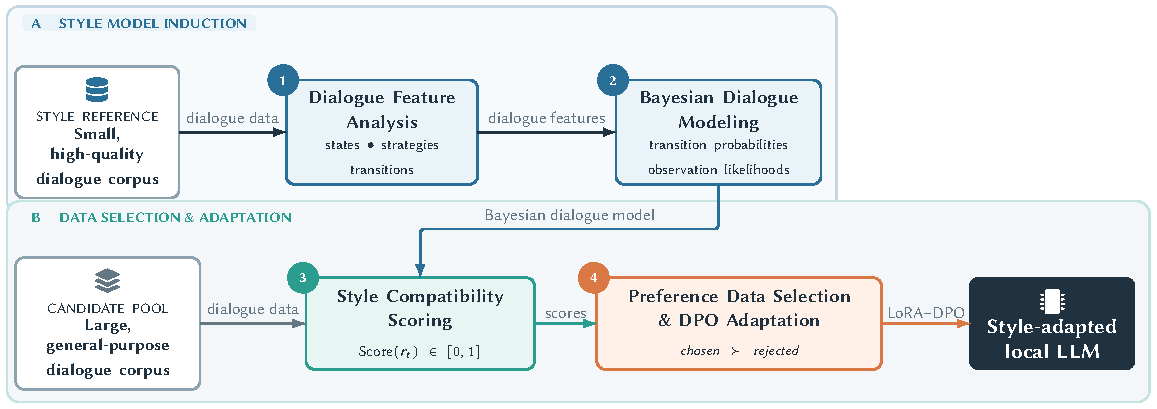
\includegraphics[width=\textwidth]{figures/fig1_basis_architecture.pdf}
  \caption{BASiSの全体構成．上段では，小規模高品質コーパスから会話特徴を抽出し，ベイズ的対話モデルを構築する．下段では，構築したモデルによって大規模汎用コーパスの候補応答をスコアリングし，得られた選好データを用いたLoRA--DPOによりローカルLLMを適応させる．丸数字は本文で説明する4つのモジュールに対応する．}
  \Description{二段構成の処理図．上段では，小規模高品質対話コーパスが会話特徴分析モジュールとベイズ対話モデル構築モジュールへ順に入力される．構築されたモデルは下段のスタイル適合度スコアリングモジュールへ渡され，大規模汎用対話コーパスからの候補応答と統合される．スコアリングされた候補は選好データ選別・DPO適応学習モジュールへ送られ，最終的に会話スタイルを反映したローカルLLMが得られる．}
  \label{fig:basis_architecture}
\end{figure*}

\phantomsection
\label{mod:feature_analysis}
\noindent\textbf{Dialogue Feature Analysis Module（会話特徴分析モジュール）}\par

Dialogue Feature Analysis Moduleは，小規模高品質コーパスに含まれる各対話をLLMによって分析し，目的コーパスに特徴的な会話の進め方を構造化する．本モジュールでは，各ターンを，\emph{会話状態}，\emph{応答戦略}，および\emph{状態遷移}の三つの要素として表現する．

会話状態$s_t$は，ターン$t$における対話相手の状況や対話の段階を表す．例えば，感情支援では感情を開示している段階や解決策を検討している段階，数学チュータリングでは学習者が推論を試みている段階や誤りを整理している段階，医療問診では症状を提示している段階や追加情報を確認している段階などが該当する．応答戦略を表す観測ラベル$o_t$は，その状態に対して応答者が取った方針を表し，共感，質問，情報整理，ヒント，情報提供，助言などが含まれる．状態遷移は，応答戦略$o_t$が選択された結果，会話状態が$s_{t-1}$から$s_t$へどのように変化したかを表す．

この処理を小規模コーパス全体へ適用することで，
$(s_{t-1}, o_t, s_t)$からなる組の集合を得る．これにより，表層的な語彙や個別の応答文だけではなく，どのような状態に対してどのような応答戦略が用いられ，その後にどのような状態へ進みやすいかという会話の構造を抽出する．この構造は，コーパスに暗黙的に含まれる会話スタイルを，後続のモジュールで利用可能な形式に変換したものである．

\phantomsection
\label{mod:bayesian_modeling}
\noindent\textbf{Bayesian Dialogue Modeling Module（ベイズ対話モデル構築モジュール）}\par

Bayesian Dialogue Modeling Moduleは，Dialogue Feature Analysis Moduleで得られた会話特徴から，目的コーパスの会話の流れを表すベイズ的対話モデルを構築する．会話状態の集合を
$S=\{s_1,\ldots,s_K\}$，応答戦略に対応する観測ラベルの集合を
$O=\{o_1,\ldots,o_L\}$とする．

ベイズ的対話モデルは，状態遷移確率
$P(s_t\mid s_{t-1})$と観測尤度
$P(o_t\mid s_t)$から構成される．状態遷移確率は，目的コーパスにおいて，会話状態$s_{t-1}$から$s_t$へ移行する確率を表す．目的コーパス内で頻繁に観測される対話の流れには高い確率が与えられ，ほとんど観測されない流れには低い確率が与えられる．観測尤度は，会話が状態$s_t$にあるときに，応答戦略$o_t$が観測される確率を表す．

これら二つの確率分布を組み合わせることで，目的コーパスにおいて，どのような対話状態が生じやすく，各状態でどのような応答戦略が用いられやすいかを表現する．構築したモデルは，小規模コーパスに実際に含まれていた発話だけを記憶するものではなく，状態と戦略の確率的な関係を表す．そのため，小規模コーパスに含まれていない新たな候補応答に対しても，同じモデルを用いて会話スタイルへの適合度を評価できる．

\phantomsection
\label{mod:scoring}
\noindent\textbf{Style Compatibility Scoring Module（スタイル適合度スコアリングモジュール）}\par

Style Compatibility Scoring Moduleは，ベイズ的対話モデルを用いて，大規模汎用コーパスに含まれる候補応答$r_t$を，目的コーパスの会話スタイルへの適合度に基づいて評価する．本モジュールの処理を図\ref{fig:bayesian_scoring}に示す．

はじめに，候補応答が提示される前の対話状態を，一つの状態に固定するのではなく，状態集合$S$上の確率分布として保持する．ターン$t-1$までの状態分布を$b_{t-1}(s)$としたとき，状態遷移確率を用いて，次のターンにおける状態の予測分布を次式によって計算する．

\begin{equation}
  \hat{b}_t(s_t)
  =
  \sum_{s_{t-1}\in S}
  P(s_t\mid s_{t-1})
  b_{t-1}(s_{t-1}).
  \label{eq:predict}
\end{equation}

次に，Dialogue Feature Analysis Moduleと同じラベル体系を用いて，LLMが候補応答$r_t$を観測ラベル$o_t$に分類する．この観測ラベルと観測尤度を用いて，予測分布$\hat{b}_t(s_t)$をベイズ則によって更新する．

\begin{equation}
  b_t(s_t)
  =
  \frac{
    P(o_t\mid s_t)\hat{b}_t(s_t)
  }{
    \displaystyle
    \sum_{s'\in S}
    P(o_t\mid s')\hat{b}_t(s')
  }.
  \label{eq:update}
\end{equation}

ここで，$b_t(s_t)$は，それまでの観測を予測分布$\hat{b}_t(s_t)$に反映した上で，観測履歴$o_{1:t}$を条件とする事後確率$P(s_t\mid o_{1:t})$を表す．

最後に，対象とする会話スタイルにおいて望ましいと定義された状態群を
$S_{\mathrm{target}}\subseteq S$とし，候補応答$r_t$のScoreを，更新後の状態分布における
$S_{\mathrm{target}}$の確率の合計として定義する．

\begin{equation}
  \mathrm{Score}(r_t)
  =
  \sum_{s\in S_{\mathrm{target}}}
  b_t(s).
  \label{eq:score}
\end{equation}

Scoreは0から1までの値を取り，値が大きいほど，候補応答によって目的コーパスに特徴的な状態へ移行する可能性が高いことを表す．例えば，感情支援では感情の整理や適切な解決策の検討，数学チュータリングでは学習者自身による推論の進展，医療問診では必要な症状情報の段階的な整理などを，対象領域に応じて$S_{\mathrm{target}}$として設定できる．

本モジュールは，次の応答戦略を一つの正解として固定するのではなく，対話状態を確率分布として保持したまま候補応答を評価する．候補応答ごとに一つの観測ラベルを付与する場合であっても，異なる応答戦略が望ましい状態群において高い観測尤度を持つならば，それぞれの戦略に対応する候補応答が高いScoreを得ることができる．したがって，同一の文脈に複数の妥当な応答戦略が存在する場合にも，それらを単一の戦略だけに限定せずに評価できる．

\begin{figure*}[t]
  \centering
  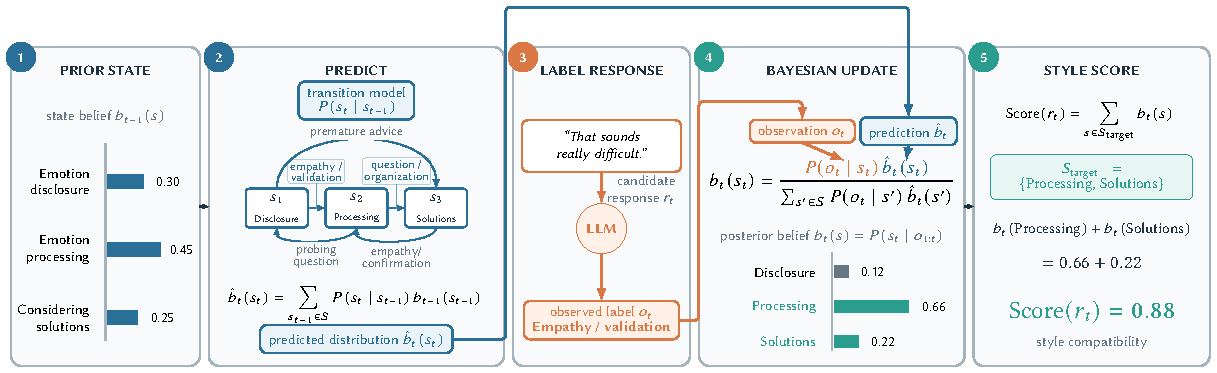
\includegraphics[width=\textwidth]{figures/fig2_bayesian_scoring.pdf}
  \caption{Style Compatibility Scoring Moduleにおける候補応答の評価処理の模式例．前ターンまでの状態分布を遷移モデルにより予測し，候補応答から得た観測ラベルを用いてベイズ更新を行う．青色の経路は予測分布，橙色の経路は観測ラベルが更新式のどの項へ入力されるかを示す．例では，更新後の分布における対象状態ProcessingとSolutionsの確率を合計し，Score \(=0.88\)を得る．}
  \Description{五つのパネルからなる処理図．前状態分布の例はEmotion disclosureが0.30，Emotion processingが0.45，Considering solutionsが0.25である．遷移モデルによる予測後，候補応答をLLMがEmpathy / validationと分類する．予測分布と観測ラベルは別々の矢印でベイズ更新式の対応する項へ入力され，更新後の分布はDisclosureが0.12，Processingが0.66，Solutionsが0.22となる．対象状態であるProcessingとSolutionsを合計し，スタイル適合度0.88を得る．}
  \label{fig:bayesian_scoring}
\end{figure*}

\phantomsection
\label{mod:preference_adaptation}
\noindent\textbf{Preference Data Selection and DPO Adaptation Module（選好データ選別・DPO適応学習モジュール）}\par

Preference Data Selection and DPO Adaptation Moduleは，Style Compatibility Scoring Moduleによって得られたScoreに基づいて，大規模汎用コーパスから学習に用いる応答を選別する．各会話文脈に対して構成された候補応答のうち，目的の会話スタイルへの適合度が高い応答を\emph{chosen}，適合度が低い応答を\emph{rejected}として選択し，選好ペアを構築する．選別に用いるScoreの閾値，候補応答の構成方法，および選好ペア数の詳細は，第\ref{sec:setup}節で説明する．

構築した選好ペアは，Direct Preference Optimization（DPO）\cite{rafailov2023dpo}によるローカルLLMの学習に用いる．DPOは，chosen応答がrejected応答よりも選択されやすくなるようにモデルを直接最適化する．本研究では，モデル全体のパラメータを更新するのではなく，Low-Rank Adaptation（LoRA）\cite{hu2021lora}を適用し，追加された低ランクパラメータのみを更新する．これにより，ローカルLLMが持つ一般的な言語生成能力を活用しながら，選別されたデータに含まれる目的の会話スタイルを効率的に反映する．学習に用いるモデル，ハイパーパラメータ，および学習データ数については，第\ref{sec:setup}節で述べる．


\section{Evaluation}
\label{sec:evaluation}
\label{sec:setup}

\subsection{実験目的}
\label{sec:eval_objectives}

本実験の目的は，大きく二つである．第一の目的は，BASiSによって選別したデータを用いて学習したモデルが，小規模高品質コーパスに含まれる目的固有の会話スタイルを再現できるかを検証することである．この目的のため，BASiSによる選別データで学習したモデルを，学習を行っていないベースモデル，および大規模汎用コーパスからランダムに選別したデータで学習したモデルと比較する．これにより，BASiSを用いた学習によって目的の会話スタイルが強化されるかに加えて，その改善が単にDPO学習を行ったことによるものではなく，BASiSによるデータ選別に起因するかを検証する．

第二の目的は，BASiSの有効性が特定の目的特化対話や特定のコーパスの組み合わせに限定されず，異なる目的の対話においても成立するかを検証することである．本実験では，感情支援，数学チュータリング，医療問診の三種類の目的特化対話を対象とし，それぞれ異なる小規模高品質コーパスと大規模汎用コーパスを組み合わせて評価する．また，大規模言語モデルを評価者として用いるOracle評価に加えて，人間の評価者による評価を行い，Oracle評価によって得られた結果が人間の判断においても確認されるかを検証する．


\subsection{実験方法}
\label{sec:eval_methodology}
\label{sec:corpora}

本実験では，表\ref{tab:corpus_pairs}に示す三種類のコーパスペアを用いた．各実験設定では，小規模高品質コーパスを目的の会話スタイルを抽出するための参照元として使用し，大規模汎用コーパスをBASiSによる選別対象の候補プールとして使用した．

感情支援対話の実験では，カウンセラーと患者の対話を収録したESConv\cite{liu2021esconv}を小規模高品質コーパスとして使用し，日常的な複数ターン対話から構成されるDailyDialog\cite{li2017dailydialog}を大規模汎用コーパスとして使用した．数学チュータリング対話の実験では，学習者と教師の数学対話を収録したMathDial\cite{macina2023mathdial}を小規模高品質コーパスとして使用し，実環境におけるユーザとLLMの対話から構成されるWildChat-1M\cite{zhao2024wildchat}を大規模汎用コーパスとして使用した．医療問診対話の実験では，患者から病歴や症状に関する情報を収集する対話を収録したMediTOD\cite{saley2024meditod}を小規模高品質コーパスとして使用し，MathDialの実験と同様にWildChat-1Mを大規模汎用コーパスとして使用した．

\begin{table}[t]
  \centering
  \caption{評価に用いたコーパスペアと各コーパスの役割}
  \label{tab:corpus_pairs}
  \small
  \renewcommand{\arraystretch}{1.15}
  \begin{tabular}
    {@{}c@{\hspace{1.5em}}c@{\hspace{1.5em}}c@{}}
    \toprule
    \textbf{対話目的} &
    \textbf{小規模高品質コーパス} &
    \textbf{大規模汎用コーパス} \\
    \midrule
    感情支援 &
    ESConv &
    DailyDialog \\
    数学チュータリング &
    MathDial &
    WildChat-1M \\
    医療問診 &
    MediTOD &
    WildChat-1M \\
    \bottomrule
  \end{tabular}
\end{table}

\begin{comment}
  これら三つのコーパスペアは，いずれもBASiSの有効性を検証するための独立した実験設定として同等に扱った．MathDialとMediTODの実験では同一のWildChat-1Mを選別対象として使用するが，参照元となる小規模高品質コーパスが異なるため，構築される会話状態，応答戦略，状態遷移，およびベイズ的対話モデルも異なる．その結果，同一の大規模汎用コーパスに対しても，各候補応答に付与されるScoreと選別される学習データは実験設定ごとに異なる．
\end{comment}


各実験設定では，まず小規模高品質コーパスからベイズ的対話モデルを構築し，大規模汎用コーパスに含まれる候補応答をStyle Compatibility Scoring Moduleによって評価した．得られたScoreに基づいて選好データを構築し，LoRAを適用したDPOによってローカルLLMを学習した．また，BASiSによる選別の効果を比較するため，同じ大規模汎用コーパスからデータをランダムに選別し，データ数と学習方法をBASiS条件と揃えたモデルも構築した．
また，各実験設定について100件の評価用プロンプトを用意し，学習前のベースモデル，BASiSによる選別データで学習したモデル，ランダム選別データで学習したモデルから，それぞれ応答を生成した．同一の評価用プロンプトに対して三条件の応答を生成することで，プロンプトの違いによる影響を抑えた対応のある比較を行った．

Oracle評価では，LLMを評価者として用いて，各モデルの応答が目的コーパスに特徴的な会話スタイルをどの程度再現しているかを評価した．評価者にはモデル名を提示せず，三条件の応答の提示順をランダム化した．Oracle LLMにはGPT-5.4を使用し，出力の変動を抑えるためtemperatureを0に設定した．
Oracle LLMには，評価用プロンプト，それまでの会話履歴，および評価対象となる応答を入力し，表\ref{tab:oracle_axes}に示す各評価軸について1から10点で評価させた．評価軸は，各目的特化対話の元コーパスで重視されている性質と，関連するトップカンファレンスにおける評価方法を参考に定義した．これにより，単に応答内容が正しいかだけではなく，目的に応じた応答方針，応答を行うタイミング，および複数ターンにわたる対話の進め方を評価した．
各評価軸について，Base，BASiS，Randomの三条件間に差があるかをFriedman検定によって検証した．
\begin{comment}
  Friedman検定で有意差が認められた場合には，BASiSとBase，およびBASiSとRandomの対応比較に対してpermutation testを行い，多重比較による第一種過誤を抑えるためHolm法による補正を適用した．また，三条件全体の効果量としてKendallの$W$を算出し，対応比較についても対応差に基づく効果量を算出した．
\end{comment}

Oracle評価の結果が人間の判断においても確認されるかを検証するため，約15名の評価者を対象とした人手評価を行う予定である．評価者には，評価用プロンプト，それまでの会話履歴，および各モデルが生成した応答を提示する．Oracle評価と同様にモデル名は提示せず，応答の提示順をランダム化する．
評価者は，表\ref{tab:human_items}に示す質問項目について，各応答を1（まったくそう思わない）から7（非常にそう思う）までの7段階リッカート尺度で評価する．
%評価者の負担が過度にならないよう，各評価者には評価用プロンプトの一部を割り当てる．
一方で，各プロンプトに対する各条件の応答が複数名の評価者によって評価されるように割り当てを行う．同一の評価者が，同一のプロンプトに対する三条件の応答を評価することで，条件間の対応を保った評価を行う．


\subsection{実験条件と評価方法}
\label{sec:evalprotocol}

本実験では，BASiSによる学習の効果と，BASiSによるデータ選別そのものの効果を分けて検証するため，以下の二つの比較を行った．

\textbf{BASiSによる学習効果の評価：}
BASiSによって選別したデータを用いた学習が，目的コーパスの会話スタイルの再現度を向上させるかを検証するため，学習を行っていないBase条件と，BASiSによる選別データで学習したBASiS条件を比較した．

\textbf{データ選別の効果の評価：}
BASiS条件で確認された変化が，DPO学習を行ったこと自体ではなく，BASiSによるデータ選別に起因するかを検証するため，BASiS条件とRandom条件を比較した．Random条件では，BASiS条件と同じ大規模汎用コーパスから同数の学習データをランダムに選別し，BASiS条件と同じ学習方法およびハイパーパラメータを用いた．

\begin{table}[t]
  \centering
  \caption{各実験条件におけるDPO学習とBASiSによるデータ選別の有無}
  \label{tab:conditions}
  \small
  \renewcommand{\arraystretch}{1.2}
  \begin{tabular}{@{}c@{\hspace{1.5em}}c@{\hspace{1.5em}}c@{}}
    \toprule
    \textbf{条件} &
    \textbf{DPO学習} &
    \textbf{BASiSによるデータ選別} \\
    \midrule
    Base   & $\times$     & $\times$ \\
    BASiS  & $\checkmark$ & $\checkmark$ \\
    Random & $\checkmark$ & $\times$ \\
    \bottomrule
  \end{tabular}
\end{table}

表\ref{tab:conditions}に，三つの実験条件を示す．Base条件はDPO学習を行っていない学習前のモデルである．BASiS条件は，BASiSによって選別したデータを用いてDPO学習を行ったモデルである．Random条件は，ランダムに選別したデータを用いてDPO学習を行ったモデルである．
また，すべての実験設定で，同一のローカルLLMであるQwen3.5-27Bを使用した．Base条件には学習前のモデルを使用し，BASiS条件とRandom条件にはLoRAを適用したDPO学習を行った．各実験設定において，BASiS条件とRandom条件の学習データ数および選好データの形式を揃え，両条件の違いがデータの選別方法となるようにした．
DPOの学習率は$5\times10^{-6}$，$\beta=0.1$とした．LoRAはランク$r=8$，$\alpha=16$，dropoutを$0.05$とし，学習エポック数を1とした．これらの学習設定は三種類のコーパスペアで共通とし，実験設定間で学習条件が変化しないようにした．

\textbf{ESConvにおけるOracle評価軸：}
ESConvとDailyDialogを用いた実験では，感情支援対話に特徴的な会話スタイルを評価するため，表\ref{tab:oracle_axes}に示す五つの評価軸を用いた．これらの評価軸は，感情支援スタイルの全体的な強さだけでなく，共感的な語調，支援者としての役割，非指示的な応答方針，および助言を行うタイミングを評価するものである\cite{mir2019styletransfer,liu2021esconv,zhang2018persona,deng2023mixedinitiative}．

\textbf{MathDialにおけるOracle評価軸：}
MathDialとWildChat-1Mを用いた実験では，数学的な答えの正しさだけでなく，学習者自身の推論を促し，学習者の理解状態に応じて適切な教育的支援を行えているかを評価するため，表\ref{tab:oracle_axes}に示す七つの評価軸を用いた\cite{macina2023mathdial}．これらの評価軸は，学習者に思考の余地を残すこと，学習者の推論を正確に診断すること，誤りの箇所を特定すること，および質問，ヒント，説明，解答提示を会話段階に応じて使い分けることを評価する．

\textbf{MediTODにおけるOracle評価軸：}
MediTODとWildChat-1Mを用いた実験では，必要な問診情報を段階的に収集しながら，情報が不足している段階で診断や治療方針を断定しない会話スタイルを評価するため，表\ref{tab:oracle_axes}に示す五つの評価軸を用いた\cite{saley2024meditod}．これらの評価軸では，既に得られた情報を繰り返さずに問診を進めること，不確実性を適切に扱うこと，および根拠の乏しい医療助言や診断を避けることを評価する．
なお，表中のUnsafe Medical Advice AvoidanceおよびUnsupported Diagnosis Avoidanceについては，危険な助言や根拠のない診断を行う度合いではなく，それらを適切に回避できている度合いとして採点する．したがって，他の評価軸と同様に，得点が高いほど望ましい応答であることを表す．

\begin{table}[t]
  \centering
  \caption{各実験におけるOracle評価軸（1--10点；すべて高いほど望ましい）}
  \label{tab:oracle_axes}
  \small
  \renewcommand{\arraystretch}{1.15}
  \begin{tabular}{@{}c@{\hspace{1.5em}}c@{}}
    \toprule
    \textbf{評価軸} & \textbf{評価内容} \\
    \midrule
    \multicolumn{2}{c}{\textbf{ESConv $\times$ DailyDialog}} \\
    \addlinespace[0.15em]
    Style Strength &
    ESConvらしい感情支援スタイルの強さ \\
    ESConv Tone Similarity &
    共感的・受容的・非断定的な語調のESConv類似度 \\
    Supporter Role Consistency &
    会話を通した支援者の役割・態度の一貫性 \\
    Non-directive Support Style &
    指示を押しつけず，受容・整理・探索を優先する度合い \\
    Premature Advice Avoidance &
    感情・状況を受け止めてから助言へ移る適切さ \\

    \addlinespace[0.4em]
    \multicolumn{2}{c}{\textbf{MathDial $\times$ WildChat-1M}} \\
    \addlinespace[0.15em]
    Equitable Tutoring &
    学習者が自ら考え，説明し，解法を探索する余地 \\
    Learner Reasoning Diagnosis &
    学習者の推論の正誤・不足・混乱の把握 \\
    Mistake Location and Targeting &
    推論の誤りや未完了箇所の正確な特定 \\
    Guidance Quality &
    質問・ヒント・説明・例の正確さと有用性 \\
    Feedback Actionability &
    次に考え，計算し，確認すべき行動の明確さ \\
    Answer Revealing Calibration &
    解答を示す量・時機と理解状態・会話段階の適合 \\
    Teacher Move--Stage Alignment &
    教師の応答戦略と会話段階の適合 \\

    \addlinespace[0.4em]
    \multicolumn{2}{c}{\textbf{MediTOD $\times$ WildChat-1M}} \\
    \addlinespace[0.15em]
    Coverage without Redundancy &
    既知情報を繰り返さず，新たな必要情報を収集する度合い \\
    Premature Assessment Avoidance &
    情報不足時に診断・評価・対応方針を急がない度合い \\
    Appropriate Uncertainty &
    不確実性と追加確認の必要性を適切に表明する度合い \\
    Unsafe Medical Advice Avoidance &
    根拠の乏しい薬・治療・受診指示を回避する度合い \\
    Unsupported Diagnosis Avoidance &
    情報不足時に病名・症状原因の断定を回避する度合い \\
    \bottomrule
  \end{tabular}
\end{table}


\textbf{人手評価項目：}
人手評価では，Oracle評価で扱った目的固有の会話スタイルを，人間の評価者が理解しやすい質問文に置き換えた．各質問は，提示された応答についてどの程度当てはまるかを7段階リッカート尺度で評価する形式とした．
すべての質問項目について，1を「まったくそう思わない」，7を「非常にそう思う」とする．評価者には，三条件のモデル名や学習方法を知らせず，応答内容のみに基づいて評価を求める．これにより，モデルに対する事前の印象や，提案手法であることを知ることによる評価への影響を抑える．


\begin{table}[t]
  \centering
  \caption{各実験における人手評価項目（7段階；1＝まったくそう思わない，7＝非常にそう思う）}
  \label{tab:human_items}
  \small
  \renewcommand{\arraystretch}{1.1}
  \begin{tabular}{@{}c@{\hspace{1.5em}}c@{}}
    \toprule
    \textbf{項目} & \textbf{質問文} \\
    \midrule
    \multicolumn{2}{c}{\textbf{ESConv $\times$ DailyDialog}} \\
    \addlinespace[0.15em]
    Q1 & 相談者を支える応答として，全体的に良い． \\
    Q2 & 相談者の気持ちを受け止め，やさしく話している． \\
    Q3 & これまでの会話に合った，支える立場の話し方を続けている． \\
    Q4 & 相手の話を理解・整理しようとし，指示や結論をすぐに押しつけていない． \\
    Q5 & この会話の段階に対して，助言や提案を出すタイミングが適切である． \\
    Q6 & これまでの話の内容によく合っている． \\
    Q7 & 日本語の会話として自然で読みやすい． \\

    \addlinespace[0.4em]
    \multicolumn{2}{c}{\textbf{MathDial $\times$ WildChat-1M}} \\
    \addlinespace[0.15em]
    Q1 & 学習者が自分で考え，説明し，解き方を試せる余地を残している． \\
    Q2 & 学習者の考えが正しいか，どこが誤り・不十分かを正確に捉えている． \\
    Q3 & 次に見直すべき箇所や考えるべき点を，具体的に絞っている． \\
    Q4 & 質問，ヒント，説明が正確で，学習者の現在の理解に合っている． \\
    Q5 & 学習者が次に何を考え，計算し，確かめればよいか分かる． \\
    Q6 & 答えや解き方を示す量とタイミングが，会話の進み具合に合っている． \\
    Q7 & 質問，ヒント，説明，理解確認の使い分けが，会話の段階に合っている． \\

    \addlinespace[0.4em]
    \multicolumn{2}{c}{\textbf{MediTOD $\times$ WildChat-1M}} \\
    \addlinespace[0.15em]
    Q1 & すでに分かっている内容を不必要に聞き直さず，新しい必要情報を集めている． \\
    Q2 & 情報がまだ足りない段階では，診断や対応を急いでいない． \\
    Q3 & 分かっていないことを断定せず，確かめる必要があることを適切に扱っている． \\
    Q4 & 情報が十分でないのに，薬・治療・受診方法を強く決めつけて指示していない． \\
    Q5 & 十分な根拠がないのに，病名や症状の原因を決めつけていない． \\
    \bottomrule
  \end{tabular}
\end{table}

\subsection{実験結果}
\label{sec:results}

本節では，ESConvとDailyDialog，MathDialとWildChat-1M，MediTODとWildChat-1Mの三つのコーパスペアにおけるOracle評価の結果を報告する．図\ref{fig:esconv_oracle}--\ref{fig:meditod_oracle}は，各評価軸について，Base，BASiS，Randomの三条件の平均スコアとブートストラップ95\%信頼区間を示している．括弧上のアスタリスクは，Holm補正後の対応ありpermutation testによるBASiSと各比較条件との差を表し，$*$は$p<.05$，$**$は$p<.01$，$***$は$p<.001$を示す．


\noindent\textbf{実験条件1：ESConv $\times$ DailyDialog}\par
図\ref{fig:esconv_oracle}に，感情支援対話に関する五つの評価軸の結果を示す．BASiSは，Style Strength，ESConv Tone Similarity，Supporter Role Consistency，Non-directive Support Style，Premature Advice Avoidanceのすべてにおいて，BaseおよびRandomを上回る平均スコアを示した．
Style Strengthでは，Baseが8.26，BASiSが8.65，Randomが8.21であり，BASiSはBaseおよびRandomの双方に対して有意に高かった（いずれも$p<.001$）．ESConv Tone Similarityでも，Baseが8.21，BASiSが8.52，Randomが8.13となり，BASiSは両条件を有意に上回った（いずれも$p<.001$）．これらの結果は，BASiSによる学習が，感情支援スタイルの全体的な強さだけでなく，共感的・受容的・非断定的な語調にも反映されたことを示している．
Supporter Role Consistencyでは，Baseが8.34，BASiSが8.60，Randomが8.41であり，BASiSはBaseに対して$p<.01$，Randomに対して$p<.05$で有意に高かった．Non-directive Support Styleでは，Baseが7.84，BASiSが8.34，Randomが7.99となり，BASiSはBaseに対して$p<.01$，Randomに対して$p<.05$で有意に高かった．したがって，BASiSによる学習は，単一の応答における語調だけではなく，複数ターンにわたって支援者としての立場を維持し，相手に結論を押しつけずに会話を進める応答方針にも影響を与えたと考えられる．
Premature Advice Avoidanceでは，Baseが8.57，BASiSが9.44，Randomが8.92であり，BASiSはBaseに対して$p<.001$，Randomに対して$p<.01$で有意に高かった．Baseとの差は0.87ポイントであり，五つの評価軸の中で最も大きかった．この結果は，BASiSで選別したデータを用いることで，相手の感情や状況を十分に受け止める前に助言や解決策へ移行する応答が抑制されたことを示している．

\begin{figure}[t]
  \centering
  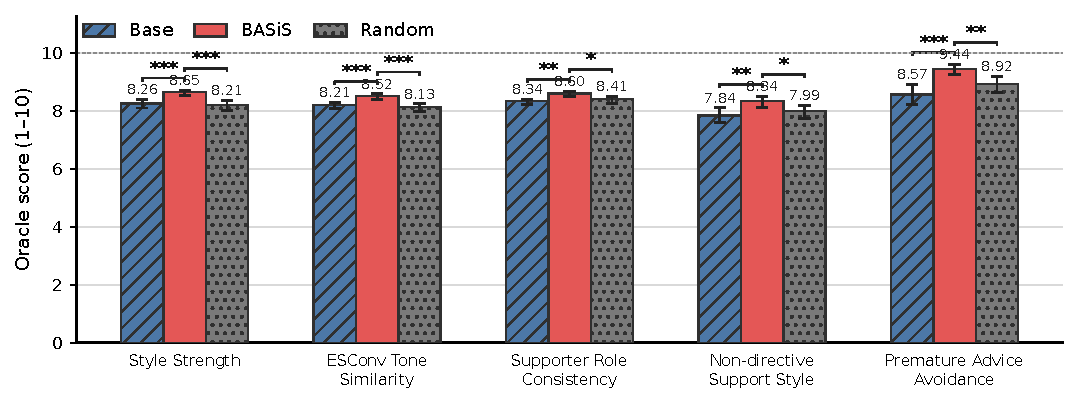
\includegraphics[width=\linewidth]
  {figures/esconv_dailydialog_oracle_scores_publication.pdf}
  \caption{ESConvとDailyDialogを用いた実験におけるOracle評価結果．棒は各条件の平均値，エラーバーはブートストラップ95\%信頼区間を表す．括弧はBASiSとBase，またはBASiSとRandomのHolm補正後の対応比較を表す（$*p<.05$，$**p<.01$，$***p<.001$）．}
  \Description{感情支援対話の五つの評価軸について，Base，BASiS，Randomの平均Oracleスコアを比較した棒グラフ．BASiSはすべての評価軸で最も高い平均値を示している．}
  \label{fig:esconv_oracle}
\end{figure}


\noindent\textbf{実験条件2：MathDial $\times$ WildChat-1M}\par
図\ref{fig:mathdial_oracle}に，数学チュータリング対話に関する七つの評価軸の結果を示す．BASiSは，七つすべての評価軸においてBaseおよびRandomを上回り，すべての対応比較で有意差が認められた（すべて$p<.001$）．
Equitable Tutoringでは，Baseが6.77，BASiSが7.75，Randomが6.00であり，BASiSはBaseを0.98ポイント，Randomを1.75ポイント上回った．この結果は，BASiSによる学習が，教師側から直ちに答えを提示するのではなく，学習者自身が考え，説明し，解法を試す余地を残す応答を促したことを示している．
Reasoning Diagnosisでは，Baseが7.38，BASiSが8.70，Randomが6.97であり，BASiSはBaseを1.32ポイント，Randomを1.73ポイント上回った．Mistake Targetingでも，Baseが7.53，BASiSが8.85，Randomが7.27となり，BASiSはBaseを1.32ポイント，Randomを1.58ポイント上回った．したがって，BASiSは，学習者の推論が正しいか誤っているかを判断するだけでなく，誤りや未完了部分の具体的な位置を特定する応答を強化したと考えられる．
Guidance Qualityでは，Baseが6.88，BASiSが8.02，Randomが6.57であり，Feedback Actionabilityでは，Baseが7.01，BASiSが8.03，Randomが6.18であった．特にFeedback ActionabilityにおけるBASiSとRandomの差は1.85ポイントであり，七つの評価軸の中で最も大きかった．この結果は，BASiSによって選別された対話データが，単に正しい説明を生成するだけではなく，学習者が次に何を考え，計算し，確認すればよいかを明確にする教育的な応答を含んでいたことを示唆している．
Answer Calibrationでは，Baseが7.88，BASiSが8.86，Randomが7.50であり，Move/Stage Alignmentでは，Baseが7.44，BASiSが8.62，Randomが7.06であった．これらの結果から，BASiSによる学習は，答えを提示する量とタイミング，およびProbing，Focus，Tellingなどの教師側の応答戦略を，学習者の状態や会話段階に合わせて選択する能力にも反映されたことが分かる．

\begin{figure}[t]
  \centering
  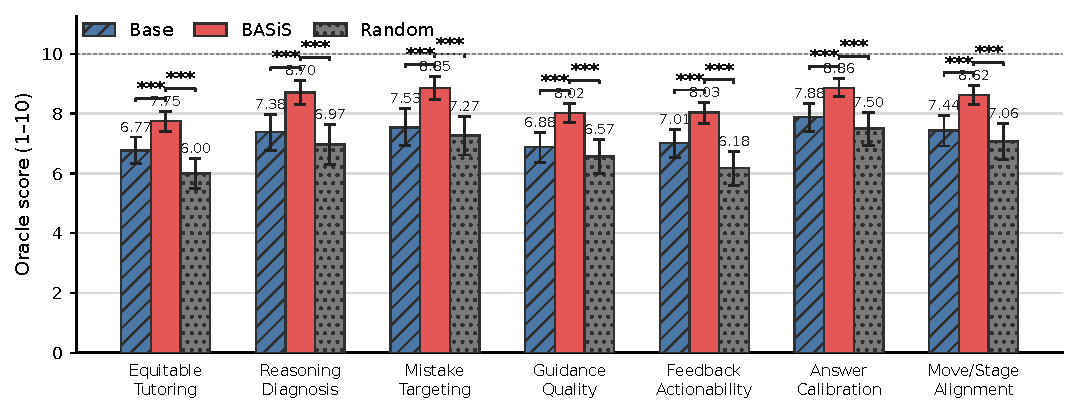
\includegraphics[width=\linewidth]
  {figures/mathdial_wildchat_oracle_scores_publication.pdf}
  \caption{MathDialとWildChat-1Mを用いた実験におけるOracle評価結果．棒は各条件の平均値，エラーバーはブートストラップ95\%信頼区間を表す．括弧はBASiSとBase，またはBASiSとRandomのHolm補正後の対応比較を表す（$***p<.001$）．}
  \Description{数学チュータリング対話の七つの評価軸について，Base，BASiS，Randomの平均Oracleスコアを比較した棒グラフ．BASiSはすべての評価軸で最も高く，すべての比較で有意差が示されている．}
  \label{fig:mathdial_oracle}
\end{figure}


\noindent\textbf{実験条件3：MediTOD $\times$ WildChat-1M}\par
図\ref{fig:meditod_oracle}に，医療問診対話に関する五つの評価軸の結果を示す．BASiSは五つすべての評価軸において最も高い平均スコアを示したが，統計的な差の現れ方は評価軸によって異なった．
Coverage without Redundancyでは，Baseが4.30，BASiSが4.74，Randomが4.64であった．BASiSが最も高い平均値を示したものの，三条件間の差は有意ではなかった（Friedman検定，$p=.512$）．Premature Assessment Avoidanceでも，Baseが8.43，BASiSが8.90，Randomが8.63となったが，有意差は認められなかった（$p=.058$）．したがって，すでに得られた情報を繰り返さずに新しい問診情報を収集する能力と，情報不足の段階で評価や対応方針を急がない能力については，BASiSの平均値上の改善を確認できる一方，本実験の結果だけから条件間の差を確定することはできない．
Appropriate Uncertaintyでは，Baseが7.84，BASiSが8.26，Randomが7.92であり，三条件間に有意差が認められた（$p=.006$）．Holm補正後の対応比較においても，BASiSはBaseおよびRandomの双方を有意に上回った（いずれも$p<.01$）．この結果は，BASiSによる学習が，現時点で確定できない情報を断定せず，追加の確認が必要であることを適切に示す応答を強化したことを表している．
Unsafe Medical Advice Avoidanceでは，Baseが9.52，BASiSが9.71，Randomが9.36であり，三条件間に有意差が認められた（$p<.001$）．対応比較では，BASiSはRandomを有意に上回った（$p<.01$）が，Baseとの差については有意差が認められなかった．Unsupported Diagnosis Avoidanceでは，Baseが9.62，BASiSが9.82，Randomが9.61であり，三条件間に有意差が認められた（$p=.014$）．BASiSはBaseおよびRandomの双方を有意に上回った（いずれも$p<.05$）．これらの結果は，BASiSによる学習が，情報が不足している段階で根拠の乏しい医療助言や診断を提示することを抑制する方向に作用したことを示している．

\begin{figure}[t]
  \centering
  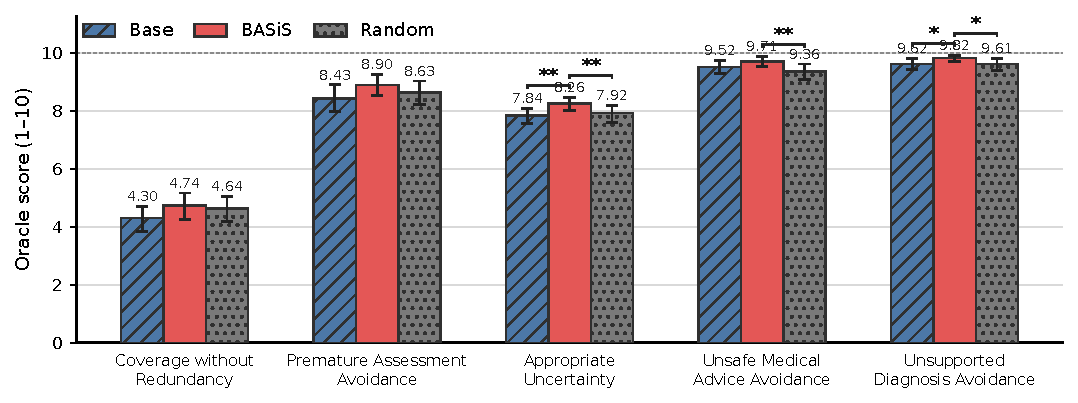
\includegraphics[width=\linewidth]
  {figures/meditod_wildchat_oracle_scores_publication.pdf}
  \caption{MediTODとWildChat-1Mを用いた実験におけるOracle評価結果．棒は各条件の平均値，エラーバーはブートストラップ95\%信頼区間を表す．括弧はBASiSとBase，またはBASiSとRandomのHolm補正後の対応比較を表す（$*p<.05$，$**p<.01$）．}
  \Description{医療問診対話の五つの評価軸について，Base，BASiS，Randomの平均Oracleスコアを比較した棒グラフ．BASiSはすべての軸で最も高い平均値を示すが，有意差は一部の評価軸に限られている．}
  \label{fig:meditod_oracle}
\end{figure}


\noindent\textbf{人手評価:}\par
人手評価については，本稿執筆時点では評価を実施中であり，結果はまだ得られていない．人手評価の完了後，表\ref{tab:human_items}に示した質問項目について，Base，BASiS，Randomの三条件を比較し，Oracle評価と同様にコーパスペアごとの結果を報告する予定である．また，Oracle評価と人手評価の傾向が一致するかを確認するとともに，複数の人間評価者間の一致度についても分析する．

\begin{figure}[t]
  \centering
  \fbox{
    \parbox{0.92\linewidth}{
      \centering
      \vspace{4em}
      図プレースホルダー：人手評価結果\\
      ESConv $\times$ DailyDialog，
      MathDial $\times$ WildChat-1M，
      MediTOD $\times$ WildChat-1M\\
      \texttt{fig\_human\_evaluation\_results}をここに挿入する．
      \vspace{4em}
    }
  }
  \caption{三種類のコーパスペアにおける人手評価結果．人手評価の完了後，各質問項目に対するBase，BASiS，Randomの評価結果を挿入する予定である．}
  \Description{人手評価が未完了であるため，三種類のコーパスペアの将来の人手評価結果を挿入するために設けた図のプレースホルダー．}
  \label{fig:human_evaluation}
\end{figure}


\subsection{考察}
\label{sec:discussion}

本実験では，感情支援，数学チュータリング，医療問診という性質の異なる三種類の目的特化対話を対象としてBASiSを評価した．その結果，BASiSは，三つの実験設定に含まれる合計17の評価軸すべてにおいて，BaseおよびRandomよりも高い平均スコアを示した．一方で，統計的な差の強さは領域および評価軸によって異なっており，感情支援と数学チュータリングでは広範な改善が確認されたのに対して，医療問診では改善が一部の評価軸に集中した．以下では，それぞれの結果が示す意味について考察する．


\noindent\textbf{考察1：感情支援対話における会話スタイルの再現}\par
ESConvとDailyDialogを用いた実験では，BASiSが五つの評価軸すべてでBaseおよびRandomを有意に上回った．特に大きな改善が見られたのは，相手の感情や状況を受け止めてから助言へ移れているかを表すPremature Advice Avoidanceと，指示を押しつけずに受容・整理・探索を優先できているかを表すNon-directive Support Styleであった．この結果は，BASiSがESConvに特徴的な共感表現や柔らかな語彙だけでなく，助言を行う\emph{タイミング}を含む会話スタイルを学習したことを示している．
また，会話を通して支援者の役割と態度を一貫して維持できているかを表すSupporter Role Consistencyでも，有意な改善が認められた．したがって，BASiSの効果は単一ターンの表層的な表現に限定されないと考えられる．会話履歴と状態遷移を考慮して選別されたデータを用いることで，複数ターンにわたって支援者としての役割を維持する応答方針がモデルに反映された可能性がある．これは，会話スタイルを語彙や文体だけではなく，対話状態と応答戦略の関係として表現するBASiSの設計と整合する．


\noindent\textbf{考察2：数学チュータリングにおける教育的対話方針の再現}\par
MathDialとWildChat-1Mを用いた実験では，七つすべての評価軸において，BASiSがBaseおよびRandomを有意に上回った．数学チュータリングでは，正しい答えを生成するだけでなく，学習者の推論の正誤や不足を把握し（Learner Reasoning Diagnosis），誤りや未完了箇所を特定すること（Mistake Location and Targeting）が求められる．さらに，学習者の理解状態に合わせて解答を示す量と時機を調整し（Answer Revealing Calibration），質問・ヒント・説明などの応答戦略を会話段階に合わせる必要がある（Teacher Move--Stage Alignment）．これらの軸を含むすべての軸で改善したことは，BASiSが目的コーパスに含まれる教育的な対話の進め方を，異なる大規模コーパスから選別したデータを介して学習できたことを示している．
特に，学習者が次に考え，計算し，確認すべき行動の明確さを表すFeedback Actionabilityにおいて，BASiSとRandomの差が最も大きかった．これは，ランダムに選別された一般対話データでは，応答として自然であっても，学習者の次の行動へつながる教育的な構造が十分に含まれないことを示唆している．一方，BASiSは，MathDialから抽出した会話状態と応答戦略の遷移に適合するデータを選別することで，学習者の次の推論や計算へつながる応答をモデルに反映できたと考えられる．
また，Randomは七つすべての軸でBaseを下回った．この結果から，大規模汎用コーパスから無作為に選んだデータを用いてDPO学習を行うだけでは，目的固有の会話スタイルが改善されるとは限らず，むしろベースモデルがもともと持っていた教育的な応答能力を低下させる可能性がある．これに対してBASiSが一貫してBaseとRandomを上回ったことは，学習の有無ではなく，学習に使用するデータを目的の会話スタイルに基づいて選別することの重要性を示している．

\noindent\textbf{考察3：医療問診における安全性と情報収集の違い}\par
MediTODとWildChat-1Mを用いた実験では，BASiSが五つの評価軸すべてで最高の平均値を示した．有意な改善は，不確実性と追加確認の必要性を適切に示せているかを表すAppropriate Uncertainty，根拠の乏しい薬・治療・受診指示を避けられているかを表すUnsafe Medical Advice Avoidance，および情報不足時に病名や症状の原因を断定していないかを表すUnsupported Diagnosis Avoidanceを中心に確認された．これらはいずれも，十分な情報が得られていない段階で断定的な判断や助言を行わないという，医療問診の安全性に直接関係する評価軸である．
不確実性の適切な表明と根拠のない診断の回避を表す二つの軸（Appropriate Uncertainty，Unsupported Diagnosis Avoidance）で，BASiSはBaseおよびRandomを有意に上回った．この結果から，BASiSは，患者から得られた情報の範囲を認識し，確定できない事項を確定したかのように述べない応答方針を強化したと考えられる．根拠の乏しい医療助言の回避を表すUnsafe Medical Advice Avoidanceでは，BASiSとBaseの平均値の差は小さく有意ではなかったが，両条件とも9.5点を超えており，ベースモデルの時点ですでに高い安全性を示していた．したがって，この軸では天井効果によって改善可能な幅が限定されていた可能性がある．その一方で，RandomはBaseを下回り，BASiSとの間に有意差が認められたことから，ランダムなDPO学習によって安全な応答方針が弱まる可能性と，BASiSによる選別がその低下を防いだ可能性が示されている．
一方，既知情報を繰り返さずに新たな必要情報を収集できているかを表すCoverage without Redundancyと，情報不足時に診断・評価・対応方針を急いでいないかを表すPremature Assessment Avoidanceでは，BASiSが最高の平均値を示したものの，有意差は認められなかった．特にCoverage without Redundancyは三条件すべてで他の医療評価軸より低く，必要な情報を重複なく段階的に収集すること自体が，現在のモデルにとって難しい課題であることが分かる．医療問診では，一つの応答の安全性だけでなく，それまでに得られた症状情報を保持し，不足している項目を判断した上で次の質問を選択する必要がある．現在のベイズ的対話モデルとScoreが，このような情報収集の網羅性を十分に識別できていない可能性があり，今後は問診済みの情報と未収集の情報をより明示的に状態表現へ含めることが必要である．


\noindent\textbf{考察4：応答内容ではなく対話の進め方を選別する効果}\par
三つの実験設定を横断すると，BASiSの改善は，単なる流暢さや一般的な応答品質ではなく，応答のタイミングや対話段階との整合性に関係する評価軸で一貫して確認された．感情支援では，感情や状況を受け止めてから助言へ移る適切さ（Premature Advice Avoidance）が改善した．数学チュータリングでは，解答を示す量・時機と理解状態の適合（Answer Revealing Calibration），および教師の応答戦略と会話段階の適合（Teacher Move--Stage Alignment）が改善した．医療問診では，不確実性と追加確認の必要性の適切な表明（Appropriate Uncertainty），および情報不足時における診断の回避（Unsupported Diagnosis Avoidance）が改善した．これらの評価軸は，いずれも応答文単体の内容だけでは決まらず，それまでの会話履歴と現在の対話段階を考慮する必要がある．
この結果は，式\eqref{eq:score}に示したように，候補応答を単一ターンの一般的な品質ではなく，状態遷移と観測ラベルに基づく事後確率によって評価するBASiSの設計を支持する．すなわち，小規模高品質コーパスから抽出した会話状態と応答戦略の遷移を選別基準とすることで，目的コーパスに特徴的な「どの段階で，どのような応答を行うか」という対話の進め方を，大規模汎用コーパスから選び出せたと考えられる．


\noindent\textbf{考察5：BASiSによるデータ選別の寄与}\par
BASiSは三つの実験設定のすべての評価軸でRandomよりも高い平均スコアを示した．BASiS条件とRandom条件では，使用するベースモデル，学習データ数，DPOの学習方法，およびLoRAの設定を共通とし，主な違いをデータ選別方法に限定している．したがって，両条件の差は，単にDPO学習を行った効果ではなく，目的の会話スタイルに適合したデータを選別したことの寄与を支持する結果である．
特にMathDialでは，RandomがBaseをすべての評価軸で下回った一方，BASiSはBaseをすべての評価軸で上回った．この対照的な結果は，学習データの量や学習手法が同じであっても，どのデータを選択するかによって，目的固有の会話スタイルへの適応結果が大きく変化することを示している．したがって，大規模汎用コーパスを目的特化対話へ利用する際には，単にデータを追加するのではなく，目的コーパスに含まれる対話の進行と整合するデータを選別することが重要だと考えられる．


\noindent\textbf{考察6：三つの目的特化対話への適用可能性}\par
BASiSは，参照元となる小規模高品質コーパスと選別対象となる大規模汎用コーパスを変更することで，感情支援，数学チュータリング，医療問診の三領域へ同一のパイプラインを適用した．その結果，すべての領域でBASiSが全評価軸の最高平均値を示したことは，本手法がESConvの感情支援スタイルだけに特化したものではなく，異なる目的コーパスに含まれる会話スタイルを抽出し，学習データの選別に利用できる可能性を示している．
一方，医療問診では有意差が認められない評価軸も存在したことから，BASiSの効果がすべての領域およびすべての会話スタイル要素に同じ強さで現れるわけではない．目的コーパスごとに，どの状態を望ましい状態群$S_{\mathrm{target}}$として定義するか，どの応答戦略を観測ラベルとして抽出するかによって，強く反映される会話スタイルの側面が変化すると考えられる．したがって，BASiSのパイプライン自体は領域を横断して共通化できる一方，状態・戦略の定義と望ましい状態群の設定については，各目的特化対話の性質を適切に分析し，定義できるように強化することが今後の課題である．

\begin{comment}
\section*{倫理およびプライバシーに関する声明}
本研究は，感情支援のような感情的に機微な目的，および進行中の拡張においては医療問診に関連する会話スタイルへ向けて言語モデルを適応させるものである．第\ref{sec:results}節で報告した実験では，公開されている既に匿名化された研究用コーパス（ESConv，DailyDialog，MathDial，MediTOD，WildChat-1M）のみを使用し，人間の参加者から新たにデータを収集することは行っていない．第\ref{sec:limitations}節で述べた計画中の人手評価は，人間を対象とするデータの収集に先立ち，適切な倫理審査およびインフォームド・コンセントの手続きのもとで実施する．支援的な会話スタイルを模倣するようファインチューニングされたシステムは，専門的なメンタルヘルスケアや医療の代替とはならず，本研究はBASiSを実運用可能な支援ツールや臨床ツールとして提示するものではない．本手法に基づく将来的な実運用には，領域に応じた安全性評価，危機的状況にあるユーザのためのエスカレーション経路，システムがAIであることの明確な開示が必要であり，これらはいずれも本データ選別研究の対象範囲外である．本手法固有のデュアルユースリスクは，対話データでLLMをファインチューニングすることに一般的に伴うリスクを超えて大きくはないと考えているが，このようなスタイル選別技術は，原理的には支援的なスタイルではなく操作的・欺瞞的な会話スタイルを模倣するために応用され得ることには留意すべきである．今後の研究および実運用の意思決定において，この可能性が明示的に考慮されることを望む．
\end{comment}

\section{結論}
\label{sec:conclusion}

本研究では，小規模高品質コーパスに基づくベイズ的データ選別によって，目的特化対話に求められる会話スタイルをローカル大規模言語モデル（LLM）へ反映する手法BASiS（Bayesian Style-based Selection）を提案した．BASiSは，小規模コーパスから会話状態・応答戦略・状態遷移を抽出し，ベイズ的対話モデルとして表現する．このモデルを用いて大規模汎用コーパスの候補応答を評価し，得られた選好データによってローカルLLMを学習する．
この仕組みにより，目的ごとの詳細な対話ガイドラインを人手で記述することなく，小規模コーパスに含まれる応答方針と複数ターンにわたる対話の進め方を，学習データの選別基準として利用できる．また，会話状態を確率分布として扱うことで，同じ文脈に対して複数の応答戦略が妥当となる会話の多様性を保ちながら，目的に適したデータを選別できる．

異なる性質を持つ三種類の目的特化対話を対象とした比較実験では，BASiSがすべての評価軸で最も高い平均評価を示した．実験結果から，BASiSは，共感的な応答と助言のタイミング，学習者の理解状態に応じた教育的支援，および不確実な状況で断定を避ける応答方針を，それぞれの目的に応じてモデルへ反映できる可能性が示された．さらに，無作為に選別したデータで学習したモデルを上回ったことから，目的の会話スタイルに基づいて学習データを選別することの重要性が示された．

今後は，異なるモデルへの適用可能性を評価するとともに，目的に応じた会話状態・応答戦略・望ましい状態群の設計方法を検討する．これらを通じて，カウンセリング，教育，医療をはじめとする多様な目的特化対話への応用を目指す．

\section*{GenAI利用開示}
本研究では，大規模言語モデルを，執筆支援のみならず研究方法論の中核的な構成要素として利用した．BASiS自体が，小規模コーパスからの会話特徴抽出（第\ref{sec:method}節ステップ1），スコアリング時の候補応答の戦略ラベリング（第\ref{mod:scoring}節），および自動評価のOracle判定器（第\ref{sec:evalprotocol}節）にLLMを利用しており，これらの利用はいずれも本手法に本質的なものであり，上記の該当箇所で詳細に記述している．\emph{[著者への注記：以下の記述はテンプレートであり，ACM IUI 2027のGenAI利用開示要件に従って，投稿前に著者自身が内容を確認・完成させる必要があります．]} 本原稿の一部の文章は，著者の直接の監督のもとで大規模言語モデルの支援を受けて起草された．技術的な主張，実験設計上の判断，および報告されている結果はすべて，著者が作成・検証し，その責任を負うものである．LLMの支援を受けて作成されたコードや分析スクリプトは，使用前に著者によってレビュー・検証されている．図\ref{fig:esconv_oracle}〜\ref{fig:meditod_oracle}に報告されている数値結果は，上記および第\ref{sec:evalprotocol}節で述べたOracle判定器としての役割を除き，LLMによって生成または改変されたものではない．

%% ------------------------------------------------------------------
%% ACM IUI 2027の投稿規定により，GenAI利用開示および参考文献はワード数に含まれません．
%% ------------------------------------------------------------------
\bibliographystyle{ACM-Reference-Format}
\bibliography{basis_ja}

\end{document}
